% summary.tex -- short version of the report (main text ~3 pages + appendix of figures).
% Build: from report/, pdflatex summary; bibtex summary; pdflatex summary; pdflatex summary
\documentclass[11pt]{article}
\usepackage[T1]{fontenc}
\usepackage[utf8]{inputenc}
\usepackage{lmodern}
\usepackage[margin=0.9in]{geometry}
\usepackage{amsmath,amssymb}
\usepackage{graphicx}
\usepackage{booktabs,tabularx,array}
\usepackage[dvipsnames]{xcolor}
\usepackage{enumitem}
\usepackage[round,authoryear]{natbib}
\usepackage[colorlinks=true,linkcolor=MidnightBlue,citecolor=OliveGreen,urlcolor=RoyalPurple]{hyperref}
\setlist{itemsep=1pt,topsep=2pt}
\newcommand{\tagP}{\textsf{\small[proven]}}
\newcommand{\tagD}{\textsf{\small[derived]}}
\newcommand{\tagE}{\textsf{\small[empirical]}}
\newcommand{\tagC}{\textsf{\small[conjecture]}}

\title{Training dynamics of tree tensor networks: summary of findings}
\author{Short version of the full report (\texttt{report/main.pdf})}
\date{October 2026}

\begin{document}
\maketitle
\vspace{-1.5em}

\paragraph{Setting.} A tree tensor network (TTN) represents a tensor $W$ by $K$ small tensors
(\emph{cores}) contracted along a tree; matrix product states (MPS, a chain), binary trees and
hierarchical Tucker (HT) trees are examples. We train $f(x)=\langle W, x_0\otimes\dots\otimes x_{N-1}\rangle$
by gradient flow on the exact population loss $\tfrac12\|W-W^*\|^2$ against a teacher $W^*$ that is a sum
of components (e.g.\ products of basis vectors), starting from random cores of scale $\sigma$. The model
is multilinear of degree $K$ in its parameters, like a deep linear network, but the tree adds structure:
a component can differ from what is already learned on only a few input positions (\emph{sites}), which
sit on a few cores. Status tags: \tagP{} theorem; \tagD{} derivation under stated assumptions;
\tagE{} measured; \tagC{} conjecture. Tens of thousands of gradient-flow runs on more than ten tree shapes; every
experimental claim was independently re-checked, except the last test in \S2.3.

\section{Headline results}

\begin{enumerate}[leftmargin=*]
\item \textbf{Small initialization gives saddle-to-saddle learning, one component at a time.} Each
plateau sits at a critical point with all bond ranks fixed, and each escape raises the rank of every
bond on a \emph{route} by one \tagE. The first plateau lasts $\propto\sigma^{-(K-2)}$, with a prefactor that
one integration of a $\sigma$-free flow computes \emph{from the initialization before training}; it predicts
the first escape time and which component wins (1,847 of 1,848 runs). The standard bound from the
initialization norm is low by up to $3\cdot10^7$ \tagP\tagD\tagE.

\item \textbf{The tree, not the size of a component, sets the later plateaus (``locality beats
weight'').} After a component is learned, the next one needs only the $k^*$ cores of the smallest subtree
connecting the cores that carry the sites where it differs (its \emph{Steiner route}). Its plateau is
absent for $k^*=1$, $\propto\ln(1/\sigma)$ for $k^*=2$, and $\propto\sigma^{-(k^*-2)}$ for $k^*\ge3$ \tagP\tagD.
Confirmed with exponent $k-2$ for $k\le5$ in about 11,600 runs on nine trees \tagE. Consequences: a
\emph{smaller} component on a shorter route is learned first as $\sigma\to0$, and the same teacher has
different plateau laws on an MPS (logarithmic) and a binary tree (power law) \tagE.

\item \textbf{The tree shape decides whether saddles are strict.} For generic (non-orthogonal) teachers,
the saddle after the first escape is strict on an MPS (logarithmic escape at the predicted rate) but
higher-order on the binary and HT trees tested, whose internal cores carry no sites (13 teachers) \tagD\tagE.

\item \textbf{Which component comes first.} If two components differ on sites carried by $\ge3$ cores,
the winner is a race fixed by the initialization direction, independent of $\sigma$ (exact at leading
order on an MPS \tagP); on two cores learning becomes greedy as $\sigma\to0$ \tagD\tagE.

\item \textbf{Failure mode: dead routes.} Under the usual fan-in initialization some routes die (an end
core decays to roundoff), stalling 18--80\% of runs with $K\ge4$ at tight bond dimension. A conserved
quantity of each route end, computed from the initialization alone, predicts it: 93\% of runs predicted
dead stall vs.\ 1.8\% of those predicted alive \tagD\tagE. Gauge-balanced initialization cannot kill leaf ends.

\item \textbf{Map of regimes.} As $\sigma$ grows: saddle-to-saddle $\to$ a rich window $\to$ lazy. A lazy
(kernel) regime exists \emph{only} if every bond reaches its cut dimension; below it training stalls on a
floor \tagD\tagE. On binary4 both boundaries scale as $\chi^{-1/2}$ \tagE.

\item \textbf{Optimizers.} GD keeps the saddle sequence below a sharp step limit
$\eta_c=2/(K s_1^{2-2/K})$ \tagP; SGD never shortens the first plateau on average, lengthens later ones and
can stall a run \tagE; Adam keeps the first component but makes the first escape $\sigma$-independent until
its $\epsilon$ restores the law \tagD\tagE; ALS, DMRG and Riemannian GD have no plateaus \tagD.

\item \textbf{Real data (MNIST, pre-registered).} The first route on a binary tree is a sibling pair
($k=3$), and across 27 pixel orders a data-only measure of short-route coupling predicts the final loss
(Spearman $-0.60$, 95\% CI $[-0.82,-0.22]$) but not the speed; spatial locality itself is not the cause
\tagE.
\end{enumerate}

\section{Theoretical results and how new they are}

\subsection{Genuinely new (no prior statement found)}
\begin{itemize}[leftmargin=*]
\item \textbf{Saddle-order theorem} \tagP{} (two independent verifications). At a saddle with one learned
component $j$ (weight $s_j$) and a spare bond channel along the route, define a ``generalized piggyback''
operator $\mathcal S$ that couples the residual through small sets of cores. If
$\lambda_{\max}(\mathcal S)<s_j$, the saddle order (lowest order at which the loss can decrease) is
\emph{exactly} $k^*$. Otherwise it drops to $2\ell^*<k^*$, with an explicit descent curve and a matching
level-wise lower bound. The condition always holds for two-component teachers learned in weight order and
for $k^*\le4$ with a definite old block, so the route rule is a theorem there; it first fails at $k^*=5$
(an MPS6 counterexample with a positive semidefinite Hessian but order 4, verified numerically to
$5\cdot10^{-4}$). Previously known: the \emph{upper} bound (a descent curve of order equal to the
rank-deficient component, \citealp{furman2026benign}) and lower bounds only for deep linear networks
\citep{achour2024loss} and one parity saddle. Prior work does not identify that the relevant set is a
Steiner subtree, which can be much smaller than the rank-deficient component.

\item \textbf{The dynamical consequence} \tagD\tagE. Where the order drops, escape is faster: a pre-registered
test (about 2,800 runs) measures exponents $2.001\pm0.001$ (order 4) and $3.996$--$3.998$ (order 6) wherever the
initialization lies below the predicted crossover, against the route law; mixed above the crossover; controls
inconclusive (dead routes). This test was \emph{not} independently verified.

\item \textbf{Route-end trap criterion} \tagD{} (verified). Which routes die is decided by a conserved
quantity per route end (its sign), so it is a property of the initialization direction; the death
probability of an end is an incomplete-beta law (0.39 at an MPS leaf end, 0.5 at the root); a route is dead
when two or more ends die (for $k\le5$); the four-core case reduces to two rotation invariants \tagP. Relates
to known shrinkage of dormant weights and imbalance-induced stalls \citep{furman2026benign}, but the
route-end condition is new.

\item \textbf{Strictness by tree shape} \tagP\tagD: a learned saddle is strict iff a two-core route exists or
a piggyback coupling exceeds $s_j$; non-orthogonal teachers create two-core routes exactly where adjacent
cores carry sites (MPS but not binary/HT).

\item \textbf{Regimes:} lazy only with full bonds; the lazy boundary constant $\sigma_{\rm lazy}\approx6.5/\sqrt\chi$
(binary4) \tagD\tagE; a $\mu$P-type parameterization for TTNs \tagD.
\end{itemize}

\subsection{TTN versions of known mechanisms (new form, not new idea)}
\begin{itemize}[leftmargin=*]
\item First escape $\propto\sigma^{-(K-2)}$ and its per-initialization blow-up time: known for homogeneous
models \citep{kumar2025early,kunin2025alternating}; new are the tree evaluation and run-by-run tests.
\item Escape laws by number of small layers (none / log / power): known abstractly \citep{rawal2026theory};
new is \emph{which} cores are small later (the Steiner route), its coupling and the closed-form head start.
\item Race vs.\ greedy order: analogous to multi-spike tensor PCA \citep{benarous2025stochastic}; new is the
classification by number of cores and the exact race on MPS.
\item GD stability limit and two-cycles (cf.\ \citealp{macdonald2025convergence}); Adam's $\epsilon$ law is
concurrent work \citep{sabanayagam2026optimizer}.
\end{itemize}

\subsection{Already known (reproduced in our setting)}
The binary tree with four sites is a depth-3 deep linear network, so its saddle sequence, greedy limit and
strict wrong-order saddles are known \citep{saxe2014exact,jacot2022saddletosaddle,achour2024loss};
balanced KKT escape directions \citep{kumar2025early}; the two-core case \citep{jiang2023algorithmic}; low
hierarchical-rank bias of hierarchical tensor factorization \citep{razin2022implicit}.

\section{Main caveats}
Results are for exact population loss and whitened Gaussian inputs, small trees ($N\le16$, mostly $N\le8$) and
mostly synthetic teachers. The large-$K$ limit of the saddle-to-saddle/rich boundary is open (a limit of 1 is
rejected for the plain model, post hoc). The real-data mechanism is a conjecture. Full scope, numbers,
error bars and the record of claims withdrawn after review are in the full report.

\bibliographystyle{plainnat}
\bibliography{references}

\clearpage
\appendix
\section{Figures (from the full report)}
\begin{figure}[h]
\centering
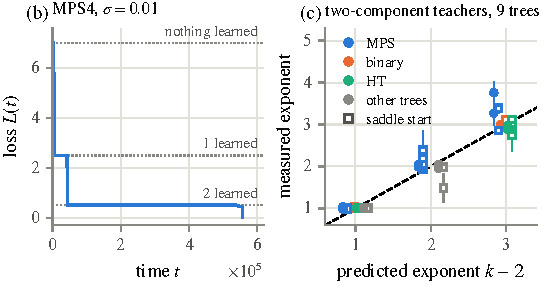
\includegraphics[width=0.95\textwidth]{figures/intro/teaser.pdf}
\caption{Saddle-to-saddle learning and the route rule (full report, Fig.~1 data panels): loss with
partial-fit plateau levels, and the measured plateau exponent against $k-2$.}
\end{figure}
\begin{figure}[h]
\centering
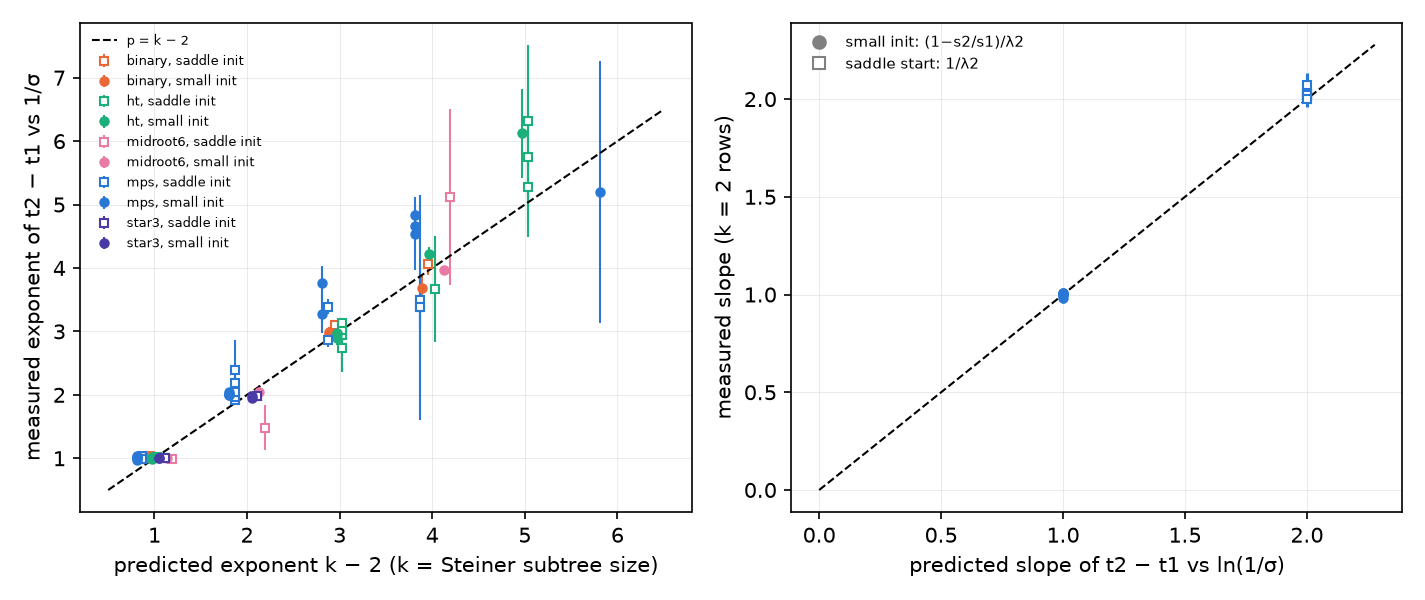
\includegraphics[width=0.9\textwidth]{figures/locality/twocomp_exponents.png}
\caption{Plateau exponent vs.\ route size $k$ across nine trees: the measured exponent follows $k-2$
(full report, Sec.~4.4).}
\end{figure}
\begin{figure}[h]
\centering
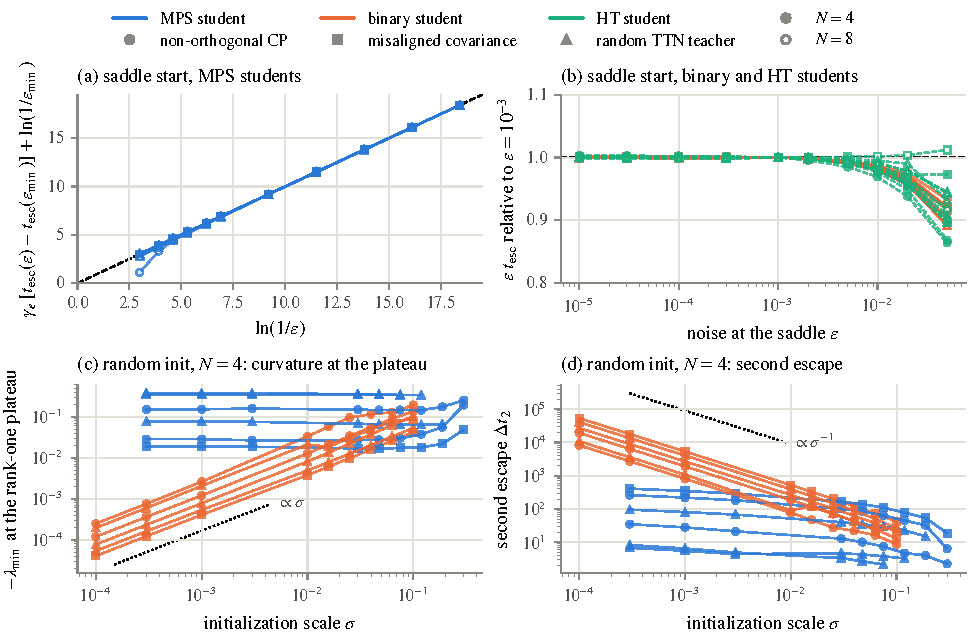
\includegraphics[width=0.9\textwidth]{figures/data_teacher/contrast.pdf}
\caption{Tree-shape contrast for generic teachers: logarithmic (strict) escape on MPS, power-law
(higher-order) on binary/HT trees (full report, Sec.~6.2).}
\end{figure}
\begin{figure}[h]
\centering
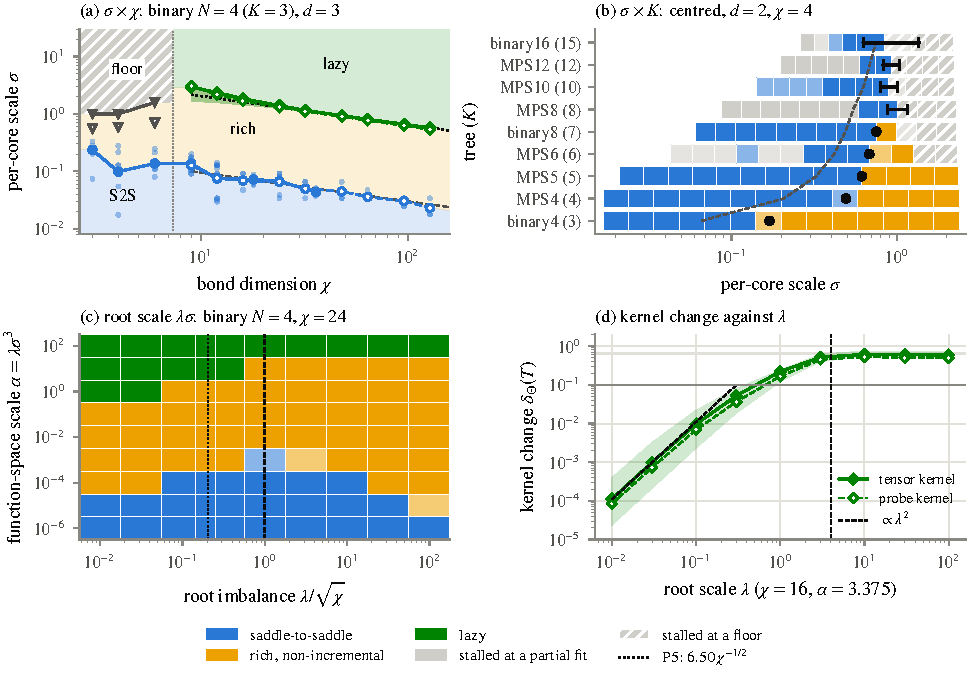
\includegraphics[width=0.85\textwidth]{figures/regime_map/map.pdf}
\caption{Map of regimes on binary4 in initialization scale $\sigma$ and bond dimension $\chi$ (full report, Sec.~3).}
\end{figure}
\end{document}
